\documentclass[tikz,border=2pt]{standalone}
\usepackage[T1]{fontenc}
\usepackage{helvet}
\renewcommand{\familydefault}{\sfdefault}
\usepackage{amsmath}
\usetikzlibrary{positioning,arrows.meta,fit,calc,backgrounds}
\definecolor{ink}{HTML}{0B0B0B}\definecolor{ink2}{HTML}{52514E}\definecolor{muted}{HTML}{898781}
\definecolor{line}{HTML}{C3C2B7}\definecolor{fill}{HTML}{F4F3EF}\definecolor{blue}{HTML}{2A78D6}
\definecolor{bluel}{HTML}{E6F0FC}\definecolor{orange}{HTML}{EB6834}\definecolor{orangel}{HTML}{FCE9E1}
\begin{document}
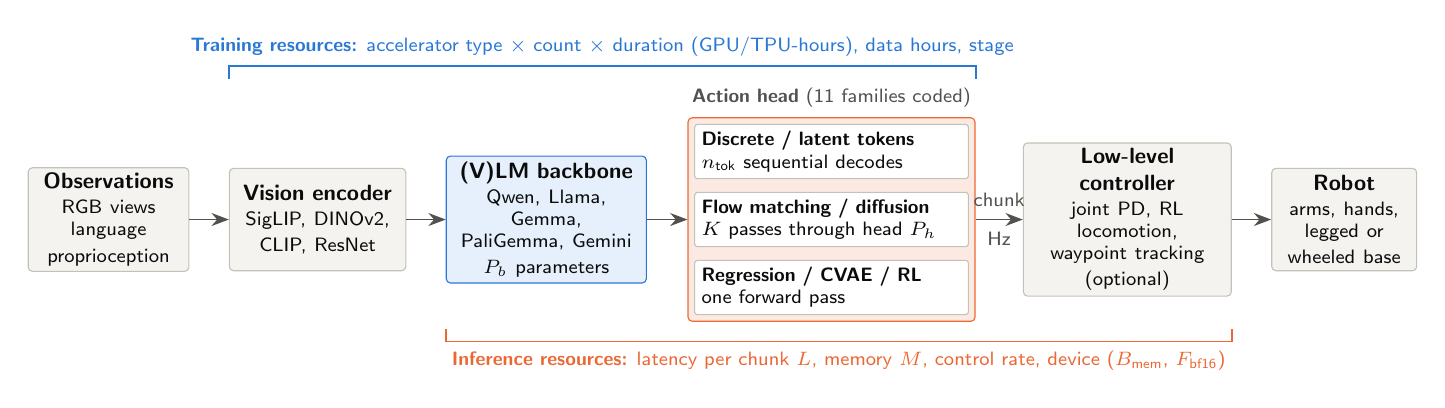
\begin{tikzpicture}[font=\footnotesize, >={Stealth[length=2.2mm]},
  box/.style={draw=line, fill=fill, rounded corners=1.5pt, align=center, minimum height=13mm, text width=#1, inner sep=2pt, text=ink},
  box/.default=21mm,
  head/.style={draw=line, fill=white, rounded corners=1pt, align=left, text width=33mm, inner sep=2.5pt, text=ink, font=\scriptsize},
  lab/.style={font=\scriptsize, text=ink2, align=center},
  arr/.style={->, draw=ink2, line width=0.6pt}]
\node[box=19mm] (obs) {\textbf{Observations}\\[1pt]\scriptsize RGB views\\ language\\ proprioception};
\node[box=21mm, right=5mm of obs] (vis) {\textbf{Vision encoder}\\[1pt]\scriptsize SigLIP, DINOv2,\\ CLIP, ResNet};
\node[box=24mm, right=5mm of vis, fill=bluel, draw=blue] (llm) {\textbf{(V)LM backbone}\\[1pt]\scriptsize Qwen, Llama, Gemma,\\ PaliGemma, Gemini\\ $P_b$ parameters};
\node[right=6mm of llm, anchor=west, yshift=0mm] (hc) {};
\node[head, right=6mm of llm] (h2) {\textbf{Flow matching / diffusion}\\ $K$ passes through head $P_h$};
\node[head, above=1.6mm of h2] (h1) {\textbf{Discrete / latent tokens}\\ $n_\text{tok}$ sequential decodes};
\node[head, below=1.6mm of h2] (h3) {\textbf{Regression / CVAE / RL}\\ one forward pass};
\begin{scope}[on background layer]
\node[draw=orange, fill=orangel, rounded corners=1.5pt, fit=(h1)(h3), inner sep=2.2pt] (headbox) {};
\end{scope}
\node[lab, anchor=south] at (headbox.north) {\textbf{Action head} (11 families coded)};
\node[box=25mm, right=6mm of headbox] (ctrl) {\textbf{Low-level controller}\\[1pt]\scriptsize joint PD, RL locomotion,\\ waypoint tracking\\ (optional)};
\node[box=17mm, right=5mm of ctrl] (robot) {\textbf{Robot}\\[1pt]\scriptsize arms, hands,\\ legged or\\ wheeled base};
\draw[arr] (obs) -- (vis); \draw[arr] (vis) -- (llm);
\draw[arr] (llm.east) -- (headbox.west);
\draw[arr] (headbox.east) -- node[lab, above, yshift=1pt]{chunk} node[lab, below, yshift=-1pt]{Hz} (ctrl);
\draw[arr] (ctrl) -- (robot);
% resource brackets
\coordinate (yT) at ($(headbox.north)+(0,6.5mm)$);
\coordinate (yB) at ($(headbox.south)+(0,-2.5mm)$);
\draw[draw=blue, line width=0.7pt] ($(vis.west |- yT)+(0,-1.6mm)$) -- (vis.west |- yT) -- (headbox.east |- yT) -- ++(0,-1.6mm);
\node[lab, text=blue, anchor=south] at ($(vis.west |- yT)!0.5!(headbox.east |- yT)$) {\textbf{Training resources:} accelerator type $\times$ count $\times$ duration (GPU/TPU-hours), data hours, stage};
\draw[draw=orange, line width=0.7pt] ($(llm.west |- yB)+(0,1.6mm)$) -- (llm.west |- yB) -- (ctrl.east |- yB) -- ++(0,1.6mm);
\node[lab, text=orange, anchor=north] at ($(llm.west |- yB)!0.5!(ctrl.east |- yB)$) {\textbf{Inference resources:} latency per chunk $L$, memory $M$, control rate, device ($B_\text{mem}$, $F_\text{bf16}$)};
\end{tikzpicture}
\end{document}
